%% 
%% Copyright 2007, 2008, 2009 Elsevier Ltd
%% 
%% This file is part of the 'Elsarticle Bundle'.
%% ---------------------------------------------
%% 
%% It may be distributed under the conditions of the LaTeX Project Public
%% License, either version 1.2 of this license or (at your option) any
%% later version.  The latest version of this license is in
%%    http://www.latex-project.org/lppl.txt
%% and version 1.2 or later is part of all distributions of LaTeX
%% version 1999/12/01 or later.
%% 
%% The list of all files belonging to the 'Elsarticle Bundle' is
%% given in the file `manifest.txt'.
%% 
%% Template article for Elsevier's document class `elsarticle'
%% with harvard style bibliographic references
%% SP 2008/03/01

% \documentclass[preprint,12pt,authoryear]{elsarticle}

%% Use the option review to obtain double line spacing
%% \documentclass[authoryear,preprint,review,12pt]{elsarticle}

%% Use the options 1p,twocolumn; 3p; 3p,twocolumn; 5p; or 5p,twocolumn
%% for a journal layout:
%% \documentclass[final,1p,times,authoryear]{elsarticle}
 \documentclass[final,5p,times,twocolumn,authoryear]{elsarticle}
%% \documentclass[final,3p,times,authoryear]{elsarticle}
%% \documentclass[final,3p,times,twocolumn,authoryear]{elsarticle}
%% \documentclass[final,5p,times,authoryear]{elsarticle}
%% \documentclass[final,5p,times,twocolumn,authoryear]{elsarticle}

%% For including figures, graphicx.sty has been loaded in
%% elsarticle.cls. If you prefer to use the old commands
%% please give \usepackage{epsfig}

%% The amssymb package provides various useful mathematical symbols
\usepackage{newtxtext,newtxmath}
\usepackage{mathtools}
\usepackage{amssymb}
\usepackage{graphicx}
\usepackage{multirow}
\usepackage{caption}
\usepackage{booktabs}
\usepackage{color, colortbl}
\usepackage[table]{xcolor}
\usepackage{amsmath}	% Advanced maths commands
% \usepackage{amssymb}	% Extra maths symbols
\usepackage{amsfonts}
\usepackage{bm}
\usepackage{float}
% \usepackage[colorlinks=true, citecolor=black, linkcolor=black, urlcolor=black]{hyperref}

\usepackage{subfig}
\usepackage{graphicx}
\usepackage{caption}
\usepackage{mwe}
\usepackage{filecontents}
\usepackage[colorlinks=true,linkcolor=blue,urlcolor=blue]{hyperref}
\usepackage{todonotes}	% todo notes
\newcommand{\tannote}[1]{\todo[inline, color=orange]{#1}}
\newcommand\mycorrections[1]{\textcolor{red}{#1}}
% \usepackage{todonotes}
%% The amsthm package provides extended theorem environments
%% \usepackage{amsthm}

%% The lineno packages adds line numbers. Start line numbering with
%% \begin{linenumbers}, end it with \end{linenumbers}. Or switch it on
%% for the whole article with \linenumbers.
%% \usepackage{lineno}
\newcommand{\mnras}{MNRAS}
\newcommand{\nat}{Nature}
\newcommand{\aj}{AJ}
\newcommand{\apj}{ApJ}
\newcommand{\apjl}{ApJL}
\newcommand{\aap}{A\&A}
\newcommand{\apjs}{ApJS}
\newcommand{\araa}{ARA\&A}
\newcommand{\prd}{Physical Review D}
% \journal{Nuclear Physics B}
\journal{Journal of \LaTeX\ Templates}
\begin{document}

\begin{frontmatter}

%% Title, authors and addresses

%% use the tnoteref command within \title for footnotes;
%% use the tnotetext command for theassociated footnote;
%% use the fnref command within \author or \address for footnotes;
%% use the fntext command for theassociated footnote;
%% use the corref command within \author for corresponding author footnotes;
%% use the cortext command for theassociated footnote;
%% use the ead command for the email address,
%% and the form \ead[url] for the home page:
%% \title{Title\tnoteref{label1}}
%% \tnotetext[label1]{}
%% \author{Name\corref{cor1}\fnref{label2}}
%% \ead{email address}
%% \ead[url]{home page}
%% \fntext[label2]{}
%% \cortext[cor1]{}
%% \address{Address\fnref{label3}}
%% \fntext[label3]{}
 %% +44 7496 472457
 
\title{Machine Learning in Fuel Consumption II: An Anomaly Detection Approach in Power Generation Plants}

%% use optional labels to link authors explicitly to addresses:
%% \author[label1,label2]{}
%% \address[label1]{}
%% \address[label2]{}
\author[p1,p1a]{J. Mulongo }  %\corref{cor2}\fnref{fn1,fn3}
\ead{jecinta.mulongo@aims-cameroon.org }
\author[p1,p2]{M. Garuti} %\fnref{fn2}
\ead{marco@aims-cameroon.org }
% \author[p1,p3]{E.P. Adzri}  %\corref{cor2}\fnref{fn1,fn3}
% \ead[url]{http://www.elsevier.com}
\author[p3]{M. Atemkeng}  %\corref{cor2}\fnref{fn1,fn3}
\ead{m.atemkeng@gmail.com}
\author[p4,p5]{T. Ansah-Narh}  %\corref{cor2}\fnref{fn1,fn3}
\ead{t.narh@gaecgh.org}

\author[p6]{Rockefeller}  %\corref{cor2}\fnref{fn1,fn3}
\ead{rockefeller@aims-senegal.org }



\author[p1,p7]{G.M. Nguegnang \corref{cor1}} %\fnref{fn1}
\ead{maxime.nguegnang@aims-cameroon.org}

\cortext[cor1]{Corresponding author}
% \cortext[cor2]{Principal corresponding author}
% \fntext[fn1]{This is the specimen author footnote.}
% \fntext[fn2]{Another author footnote, but a little more longer.}
% \fntext[fn3]{Yet another author footnote. Indeed, you can have
% any number of author footnotes.} SPACE AND ATMOSPHERIC

% RESEARCH GROUP


\address[p1]{Mathematical Sciences (AIMS-Cameroon)}
\address[p1a]{Maseno University }

\address[p4]{Centre for Radio Astronomy \& Astrophysics, Ghana Space Science and Technology Institute, Ghana Atomic Energy Commission, P. O. Box LG 80, Legon - Accra, Ghana}

\address[p5]{Space \& Atmospheric Research Group, Ghana Space Science and Technology Institute, Ghana Atomic Energy Commission, P. O. Box LG 80, Legon - Accra, Ghana}



\address[p2]{University of Padova}


\address[p3]{Rhodes Centre for Radio Astronomy Techniques \& Technologies(RATT)}
\address[p6]{Mathematical Sciences (AIMS-Senegal)}
\address[p7]{University of Yaounde 1} 


\begin{abstract}
%% Text of abstract
High fuel consumption is experienced in telecom based stations. In this paper, we show the use of supervised machine learning classification based techniques in detecting anomalies associated with the fuel consumed dataset from the base station using the generator as a source of power. We made use of classification based techniques to train
the dataset, these include support vector machines (SVM), k-nearest neighbor (KNN), logistic regression (LR), and multilayer perceptron (MLP). The aim of the study is to detect anomalies in the recorded data by learning the pattern of the fuel consumed dataset and compare the performance of the four classification techniques on the unseen dataset.  We evaluate models performance using K-fold
cross validation and training test split techniques. Performance metrics such as area under Receiver Operating Characteristic curve (ROC), the area under the precision-recall curve, accuracy, F1-measure, and so on were used to evaluate the fitted models. Comparative study of the classifier is done for model selection, and the result of this study shows that MLP has the best performance in the evaluation measured used with a score of $0.96$ in both K-fold cross validation and train test split techniques. In the area under the ROC and precision-recall curve, the model attained a score of $1.00$ and $0.98$ respectively.


\end{abstract}

\begin{keyword}
% %% keywords here, in the form: keyword \sep keyword
% 
% %% PACS codes here, in the form: \PACS code \sep code
% 
% %% MSC codes here, in the form: \MSC code \sep code
% %% or \MSC[2008] code \sep code (2000 is the default)
Anomalies \sep Multilayer  Perceptron \sep K-Nearest Neighbor   \sep Support Vector Machines \sep Logistic Regression\sep Machine Learning \sep Classification
\end{keyword}

\end{frontmatter}

\section{Introduction} \label{sec:intro}

The expansion of mobile services of the telecom industries has resulted in the installation of cell towers to diverse parts of the world. In developing countries like Cameroon, the supply of the power grid is irregular and the network companies find it difficult to manage their base stations particularly, their data centers and other IT equipment. Due to this, the management of the base stations uses diesel generators, solar panels, batteries and another secondary source of power as a backup plan to keep running their systems. However, these other power sources have also generated other problem, specifically, fuel pilferage from those who have access to fuel distribution in the various base stations and also, from other people in the vicinity and high fuel consumption as a result of the generator malfunctioning.

With an objective to provide base station management service such as refueling and site maintenance, TeleInfra\footnote{{\tt http://www.art.cm/en/node/3111}} company in Cameroon faces the problem of electricity shortage hence the company had a generator as an alternative source of power. The company works with an objective is to provide management services such as site maintenance and refueling of generators in the base stations. Like any other power dependence company in Africa, 
the company faces the problem of electricity shortages and hence, chooses to have a generator as a main back up plan. The main goal of this paper is to use machine learning (ML) techniques to learn the pattern of the fuel consumed by generator power plants in the 
TeleInfra\footnote{{\tt http://www.art.cm/en/node/3111}} company in order to observe some outliers produced by the system. The dataset used in this paper is obtained from  base stations  under supervision of TeleInfra company. It contains attributes of fuel consumed by the generators and other informations such as maintenance details.

Anomaly in a data is considered as an observation which do not conform to the expected standard in the data. Meanwhile, recent works in anomaly detection such as fraud detection analysis~\citep{2017arXiv170601953Z, chouiekh2018convnets}, 
thermal power plant~\citep{banjanovic2017neural}, medical image analysis~\citep{taboada2009anomaly}, etc., have shown how well ML techniques can be used to address these challenges.
% \indent 
From the various anomalies detection research, the algorithms used can outperform each other based on the type of data 
and the underlying assumptions employed. From the literature, most of the competitive ML techniques used in classification task like in our case, consist of SVM, KNN, LR, and MLP. In this study, we do a comparative analysis of the performance of these classifiers to determine the best classifier that can accurately detect the anomalies in the fuel consumption dataset. SVM aims in generating an optimal hyperplane that maximizes the margin between two class, that is, in the case linearly separable binary classification whereas KNN  stores the training data and predict the test instance based on distance measure and the majority votes from the training sample. LR uses probabilities to predict the chance of a sample to belong in a certain class. MLP learns the complexity of data and optimizes the weights to minimize classification error. A more detailed explanation of these classifiers is given is Section~\ref{sec:med}.
 
The rest of this paper is organized as follows: Section \ref{sec:expl} describe the dataset, feature selection and descriptive findings from the data. Section \ref{sec:med} we describe machine learning methods used in the study. Section \ref{sec:resu} we conclude the results and finding from the study discussed with comparative analysis performance of the methods used.



\section{EXPLORATORY DATA ANALYSIS}  \label{sec:expl}

\subsection{Dataset} \label{sec:desc}

The dataset is collected from the base stations powered mainly by the generator. It has 32 features both numerical and categorical data with a sample size of $5905$ inputs of the fuel consumed within September $2017$ to September $2018$. The variables used to fit the models were rescaled to ensure all the features have the same treatment. The dataset contains details of fuel consumed by generator and maintenance report made on the generator. This information recorded includes the working hours of the generator, the rate of consumption, fuel consumed, the quantity of fuel added in the generator and so on.

The important features used to fit the models were selected using the
Gradient Boosting Classifier (GBC) to reduce the number of features that do not impact the model performance. Compared to other feature selection technique such as random forest, GBC has been preferred to fit feature importance due to its ability to minimize bias and overfitting. This has been achieved in gradient boosting at error correction which is done based at every stage hence optimizing the objective function. From Figure \ref{fig:feature}, the running time of the generator, which is the number of hours the generator is working has a great influence on the output and as from Figure \ref{fig:rr} how long the generator is working per day has a positive correlation with fuel consumed. Daily fuel consumed and consumption\_HIS variables gives the fuel consumed per day and fuel consumed per period before the next refueling is done respectively. Other features such as generator capacity, maximum fuel the generator can take in one day, the rate of consumption and so on, have less information about the classification output class. The variables considered to fit the model included variables with at least $20\%$ relative importance. Figure  \ref{fig:feature} shows feature importance fitted  using Gradient Boosting classifier.
	  
 \begin{figure}[H]
      \centering
      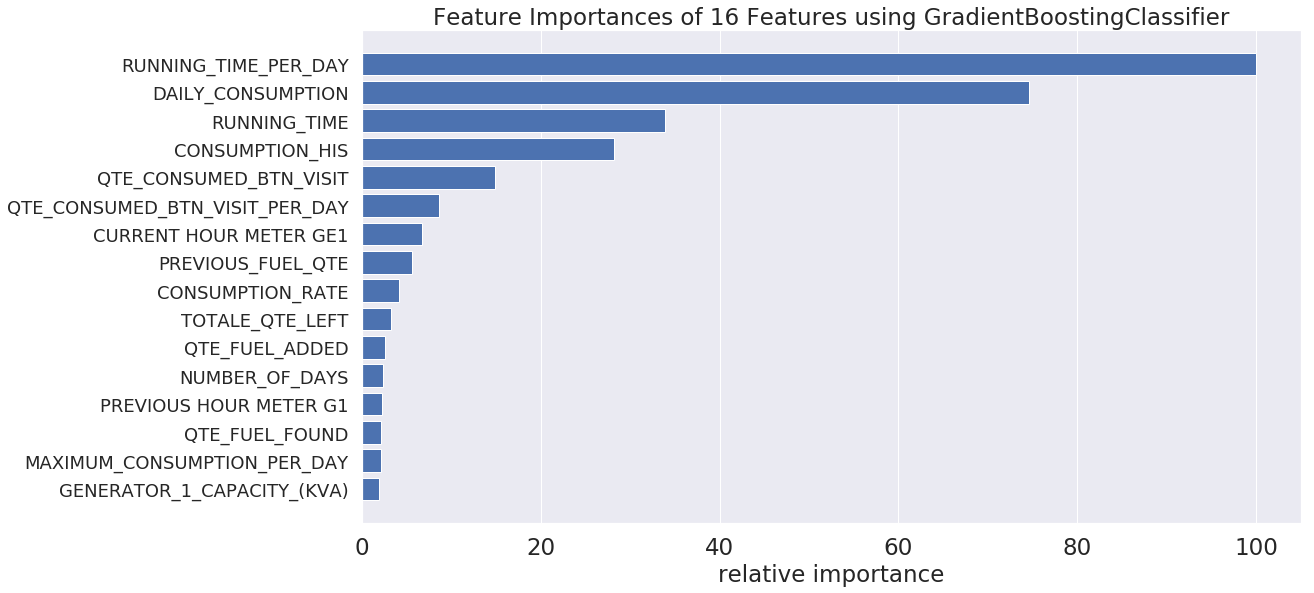
\includegraphics[width=0.55\textwidth]{Figures/Feature_importance} 
    
     \caption{Feature importance ranking fitted using Gradient Boosting classifier }
    \label{fig:feature}
   \end{figure} 
From a total sample of $5905$, $35.11$\%  of the sample were labeled as anomaly class and the rest as a normal class. The classification classes labeling was done based on the anomalies observed in the dataset.  Anomalies in the data observed include outliers, wrong entry on the number of hours the generator was working in a day, consumption per day exceeding maximum consumption the generator can take in a day and generator fuel reducing when the generator was not working. All these observations was considered to label the classification class as either normal consumption or anomaly. 

Class imbalance is a problem that highly affects classification base task. This is where the number of one class is significantly large compared to the other class. The effects of class imbalance are seen in the performance measure such as accuracy whose computation depends on both classes i.e., normal and anomaly class \cite{awoyemi2017credit}. A corrective measure of class imbalance have been proposed, that is, the use of sampling method \cite{brownlee2016master}. Sampling method can be classified as either undersampling or oversampling.  Oversampling methods involves duplicating minority class to add more inputs so as to have equal sample size as to that class with the majority sample. On the other side, undersampling involves reducing the majority of data to have the same sample size as a minority.
 
%\tannote{Class imbalance affects most classification algorithms \cite{awoyemi2017credit}. Majority class can overtake the algorithm making 
%it predict only one class with high accuracy. \cite{brownlee2016master} Class imbalance is corrected by either under-sampling of legit class, 
%that is, reducing the size of the legit observations into the same size as the fraudulent class or oversampling of the fraudulent class by making 
%a duplicate observations of the anomaly class to level both classes into the same sample size.
%Data labeling was done based on the anomalies found in the dataset. Supervised anomaly detection were applied using classification techniques and 
%therefore, the data point in the dataset were labeled as whether anomaly or normal. \\
%1. What's Class imbalance \& legit class? \\
%2. You can't cite like this:  \cite{brownlee2016master} Class imbalance is corrected ..}

%%


\subsection{Descriptive Analysis}

Gaussian distribution of fuel consumed in Figure \ref{fig:probitplot} shows the probability frequency distribution of the random variables. The fuel consumed by generator has asymmetry normal distribution with mean $261.80$ and standard deviation of $175.06$. Large variance is as a result of dispersion and the skewness of the fuel consumed data. Classifiers assumes the underlying distribution of the dataset hence the distribution has a great impact on the performance of classifiers \cite{japkowicz2011evaluating}. 
Figure \ref{fig:probitplot} shows the kernel density estimation and normal probability plot for the fuel consumed dataset. 
\begin{figure}[H]
	\centering
	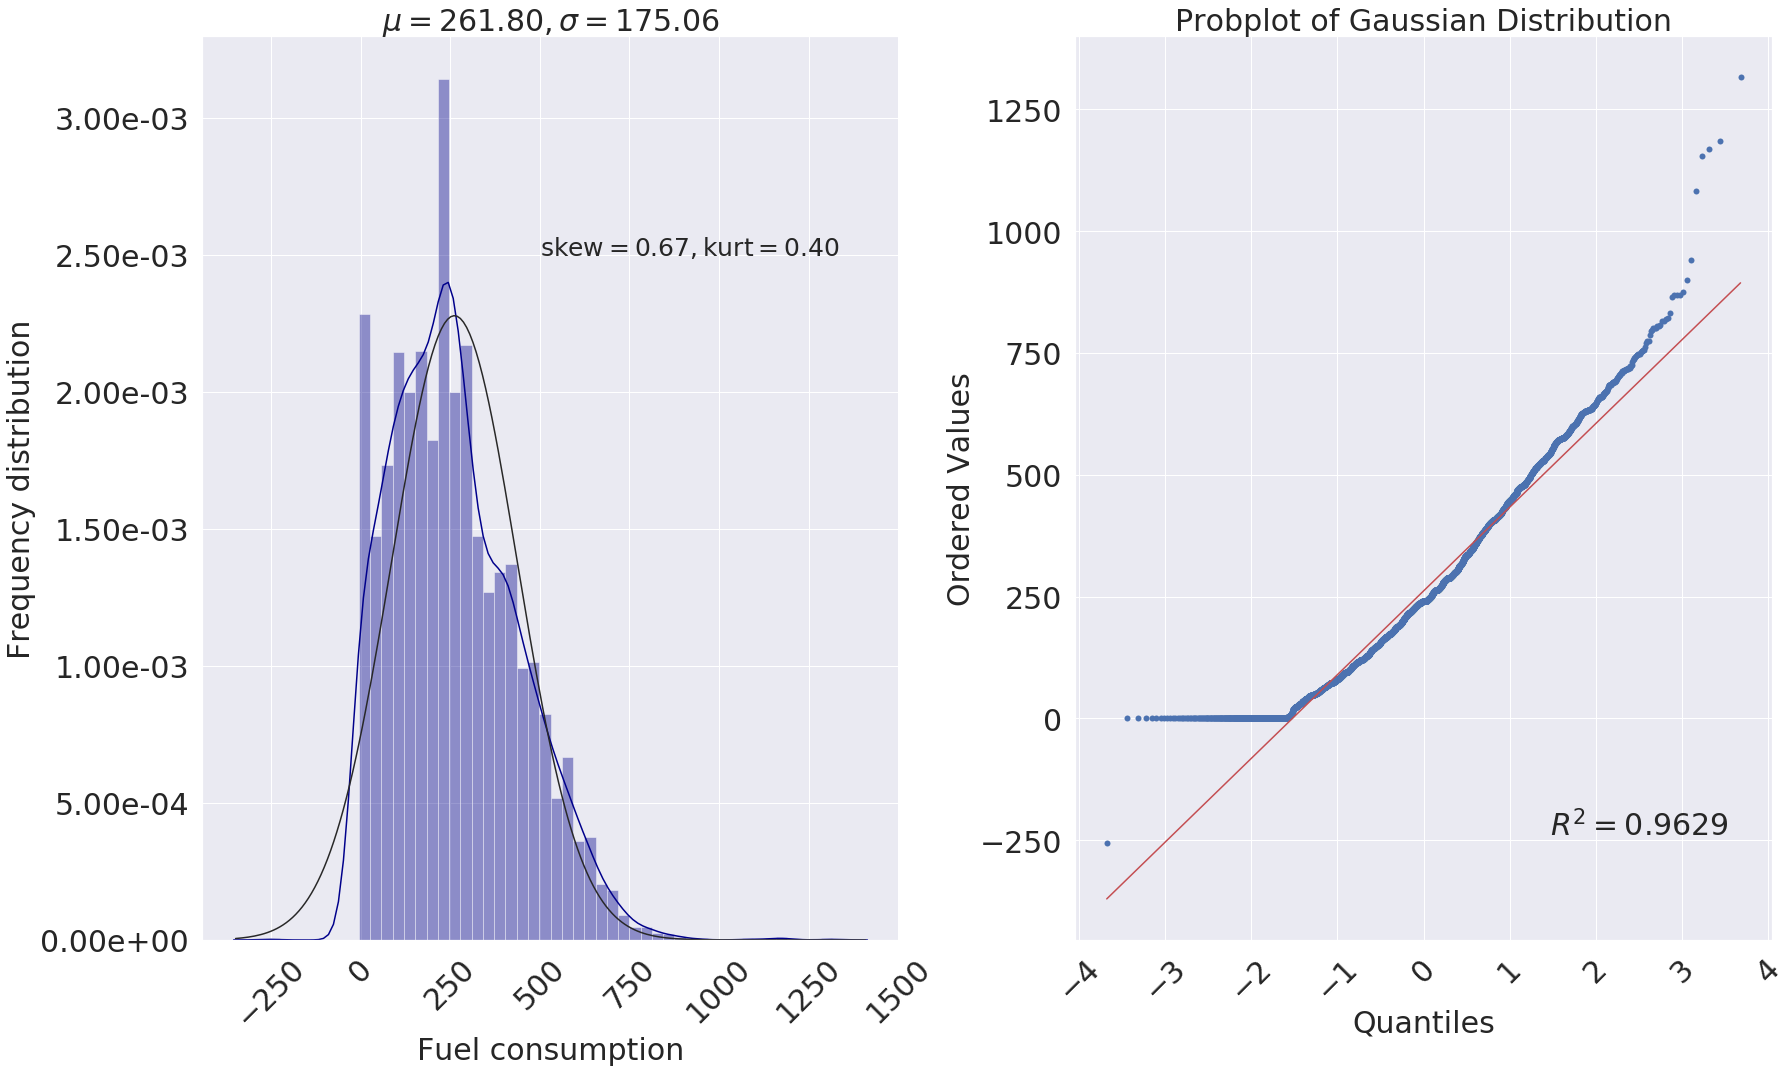
\includegraphics[width=1.0\linewidth]{Figures/probitPlot}
	\caption{Average distribution of the fuel consumed}
	\label{fig:probitplot}
\end{figure}

%
%\begin{figure*}
%   \begin{minipage}[H]{\linewidth}
%      \centering
%      \includegraphics[width=1.0\textwidth]{fig/normalcurve} %
%    \end{minipage}
%     \caption{Average distribution of the fuel consumed}
%    \label{fig:normalcurve}
%   \end{figure*}
   
% \begin{figure}[tbph]
% 	\centering
% 	\includegraphics[width=1.2\linewidth]{normalcurve}
% 	\caption{Kernel density estimation and Gaussian distribution of fuel consumed}
% 	\label{fig:normalcurve}
% \end{figure}\\
From the work done by \cite{maxime2018} on prediction of fuel consumption on the same dataset with all anomalies put into consideration, the mean of the fuel consumed within the period is $289.04$ litters with a standard deviation of $160.09$. The mean improvement is a result of the zero consumption and fuel consumption with anomalies  not taken into consideration.
The fuel consumed is positively skewed with a skew of  0.40. From Figure \ref{fig:probitplot}, the Gaussian distribution plot show that the dataset has outliers, as a result of this, the normal distribution curve deviating from the mean. From Figure \ref{fig:probitplot}, zero consumption of fuel consumed entries in the dataset causes the normal curve to start above the normal line. Due to this, the zero consumption samples were compared with the difference between what was left in the generator previously visit and what was found in the generator to make sure that consumption was actually zero fuel. As a result of the outliers, the normal distribution curve of the fuel consumed is shifted to the left, this contributes to the skew distribution of the fuel consumed. 

Figure \ref{fig:correlation matrix} displays a correlation matrix between numerical variables in the dataset. Correlation is a normalized covariance with its values ranges from $-1$ to $1$. The matrix measures a linear relationship between variables with $-1$ indicates two variables have a strong negative relationship, that is, as one variable increases the other one decreases and $1$ indicates strong positive relation, that is, an increase in one variable results to increase in the other one. The diagonal values indicate the correlation of a variable with itself. From Figure \ref{fig:correlation matrix}, fuel consumed have strong positive relation of $0.83$ with the number of hours the generator. This is explained as fuel consumed by the generator increases depending on how long the generator is working. The quantity of fuel added and the fuel consumed has a positive correlation coefficient of $0.14$. The rate at which the generator consumes fuel has positive correlation of $0.31$ with the consumption. The classification class which is the output variable has also positive correction of $0.027$  with fuel consumed. A shortcoming of the correlation matrix is that, variables with non-linear relationship the correlation matrix might not detect. 

\begin{figure}[H]
      \centering
      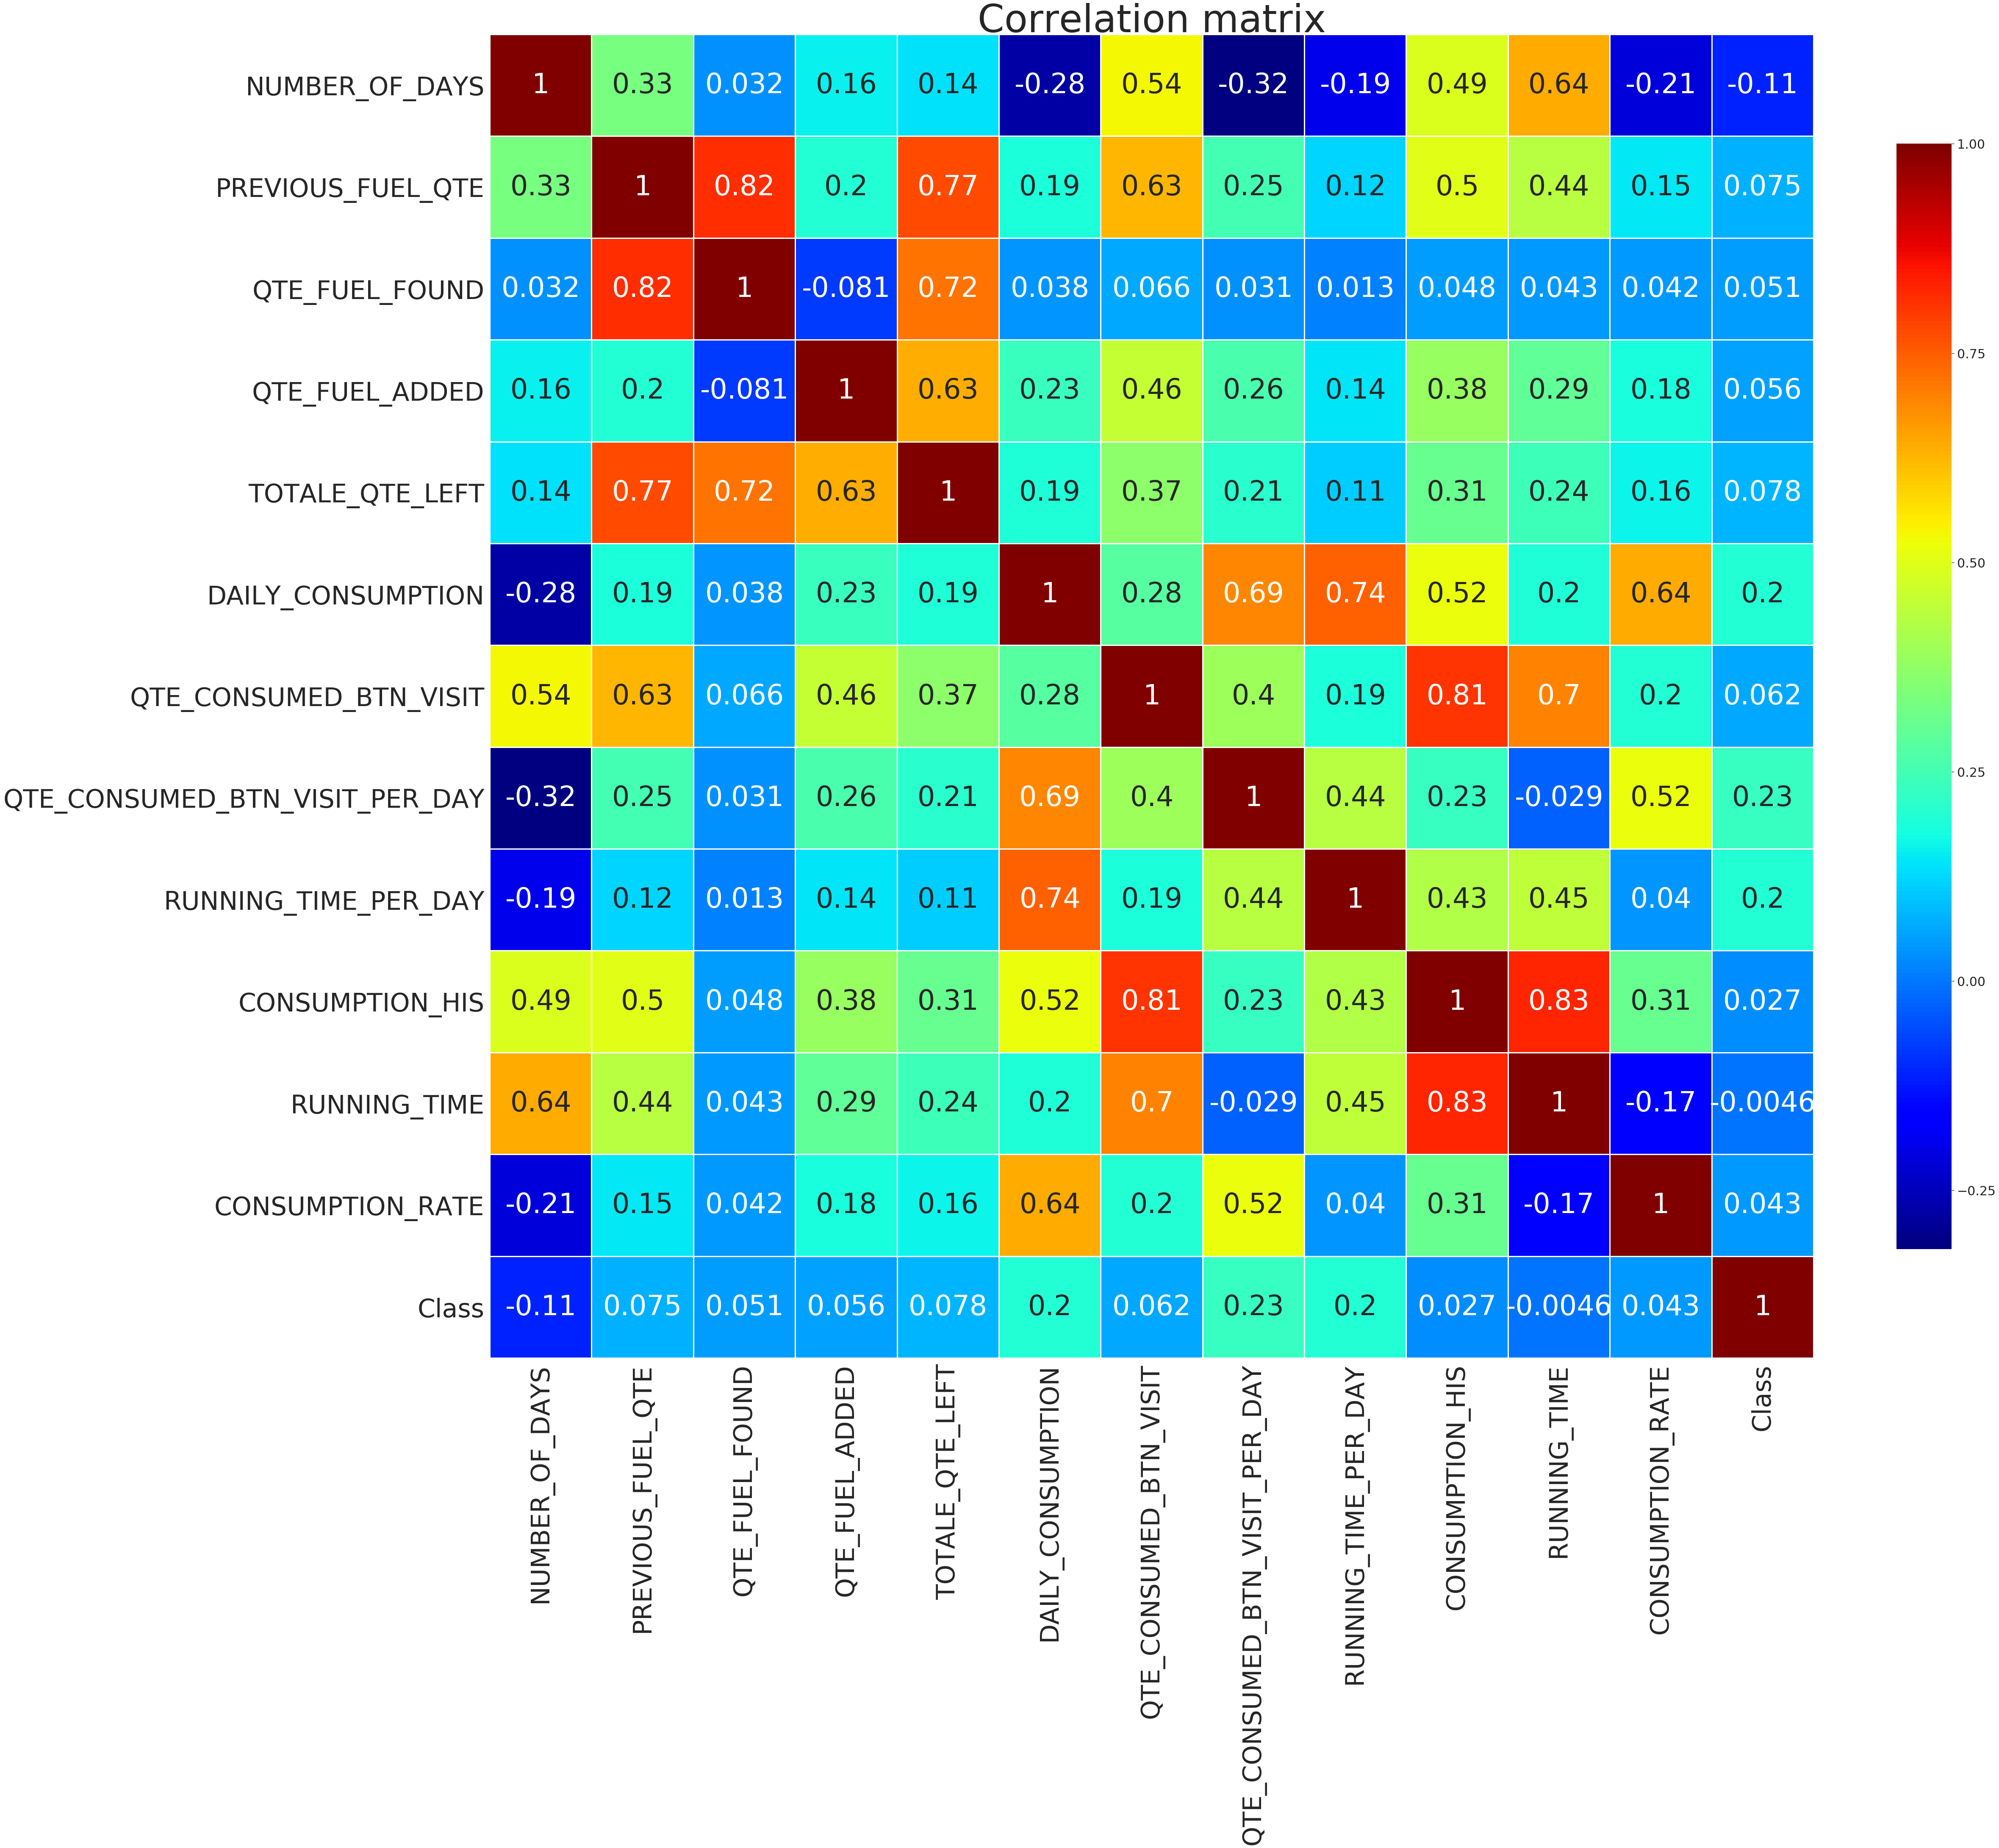
\includegraphics[width=0.55\textwidth]{Figures/correlation_matrix} %
   
     \caption{Correlation Matrix of features}
    \label{fig:correlation matrix}
   \end{figure}

The anomalies detected in the data include hours the generator was working in one day, consumption exceeds what fuel generator can consume in one day and the case where generators consume fuel and running time is zero and outliers. The anomalies discovered in the dataset were used to generates a classification class of the samples as either normal or anomaly consumption. 

Figure 	\ref{fig:boxplot} shows the distribution of fuel consumed.
\begin{figure}[H]
	\centering
	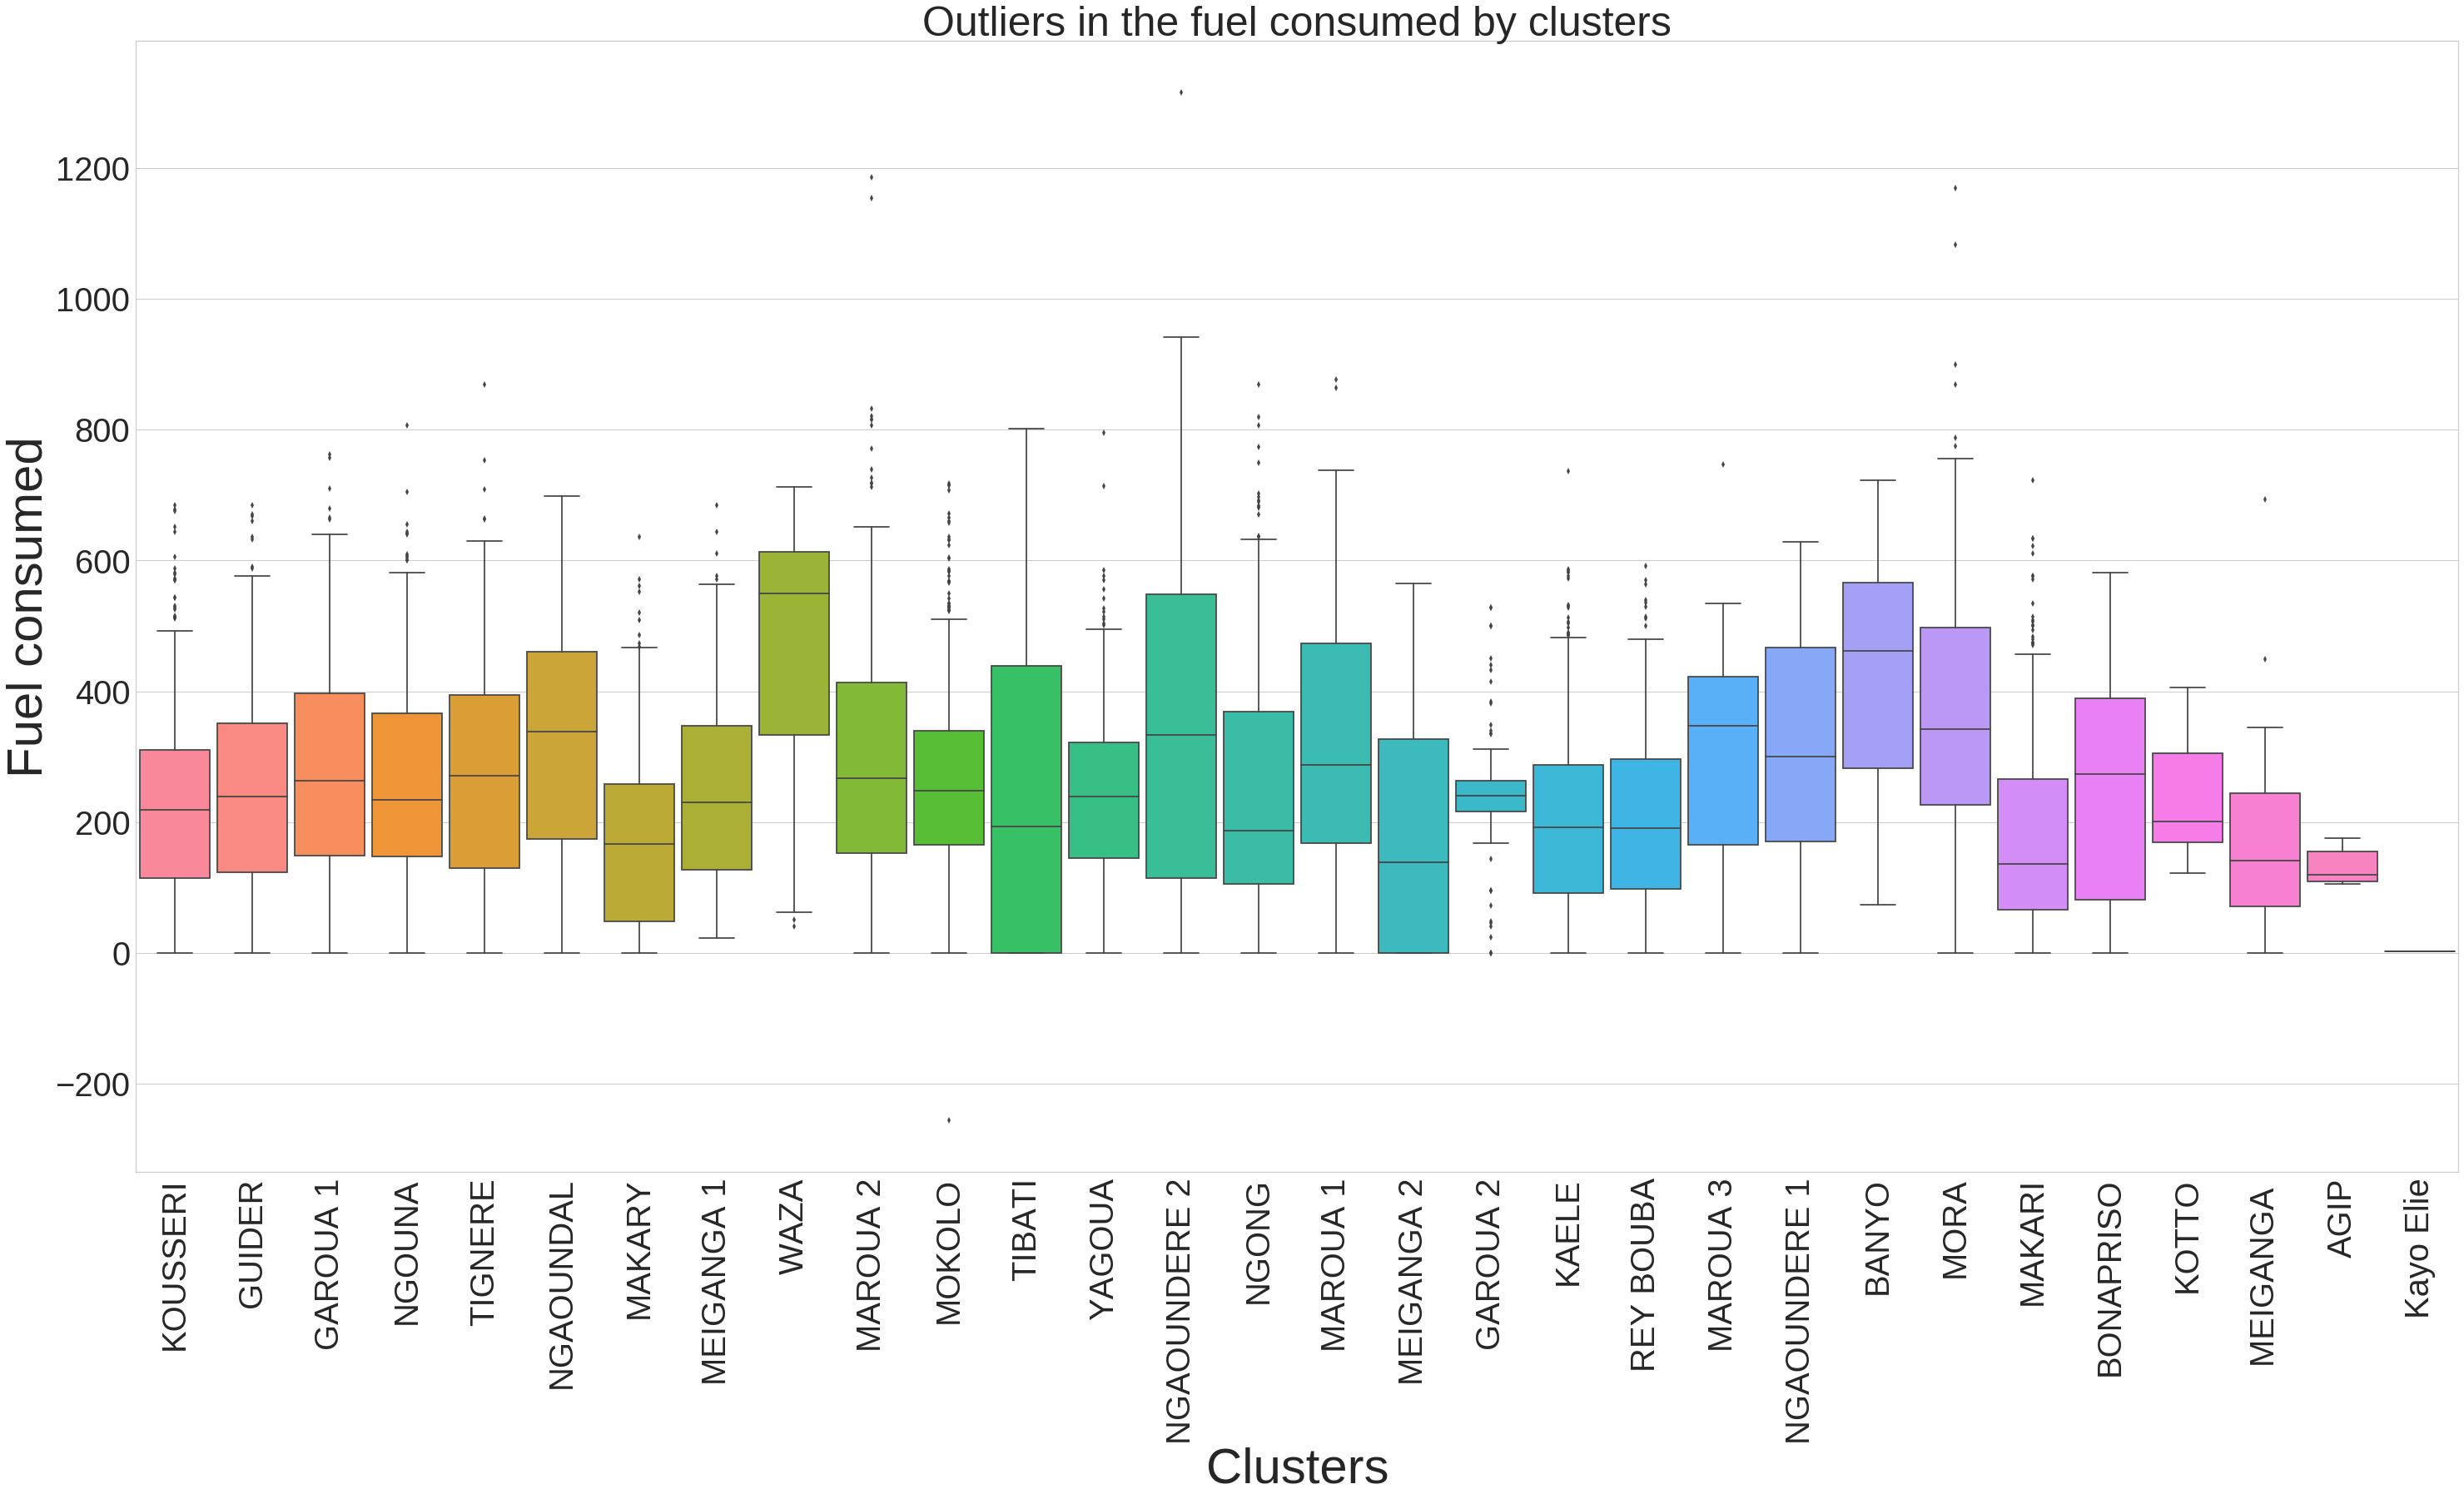
\includegraphics[width=1.1\linewidth]{Figures/Boxplot.png}
	\caption{Fuel consumed per cluster.}
	\label{fig:boxplot}
\end{figure}
A cluster is a group of sites where generators are located. Each site has a generator and therefore the fuel consumed by a cluster is the total fuel consumed by different generators in various sites. Clusters shows variation of the fuel consumed with median of the fuel consumed in most clusters ranges between $200$ and $400$. To label  a sample in the dataset as an anomaly,  the maximum consumption of each generator was considered. 

The graph below shows a plot of the number hours generator was working in one day. From the graph, recorded data indicates anomalies of working hours was more than twenty hours in one day.\\

\begin{figure}[H]
	\centering
	\includegraphics[width=1.0\linewidth]{"Figures/Generator_Working hours_per_graph"}
	\caption{Graph of number of hours the generator function in one day.}
 \label{fig:rr}
\end{figure}

From Figure    \ref{fig:rr}, the running hours of most of the generator per day fluctuates around $18$ to $25$hours in a day. An observation with more than 24hours per day was considered as an anomaly.

\section{METHODOLOGY} \label{sec:med}
\subsection{Support Vector Machines  (SVM)}\label{SVM}
Support Vector Classifier is a classification algorithm used to separate two or more class by finding a hyperplane which maximizes the margin between classes. In the case of two separable class, a decision boundary separates two class with the widest margin. When the two class are linearly separable, the ideal hyperplane is the one with the widest margin between the boundary of two classes \cite{friedman2001elements}. Given a paired of learning examples of $m$ number of features and corresponding class;   
\begin{equation}\label{eqn3}
\left\lbrace   x_{i},d_{i}\right\rbrace , i = 1 \cdots N.
\end{equation}
where $x_{i}$ are input examples and $d_{i}$ the classification class. The classifier find a function that correctly maps each input variable $x_{i}$ to its corresponding class $ d_{i} \in \{ -1, 1\}$. 
\begin{equation}\label{eqn4}
f(x) = \textbf{W}^{T}X + b = 0.
\end{equation}
$\textbf{W}$ is the weight vector and $b$ the bias. Equation \eqref{eqn4} is a decision boundary determining the class of the input variable. The support vectors, that is, the samples on the boundary of the margin determines the decision boundaries. If the function of Equation \eqref{eqn4} is greater than zero then the input variable belongs to class $1$ otherwise it belongs to class $0$. To get  an ideal hyperplane between the two classes is as same as minimizing the norm of the weight vector \cite{friedman2001elements}. For two-class classification, the input variable is either on the positive or negative side of the decision variable, such that;
\begin{equation}
d_{i}(W^{T}x_{i} + b)\geq 1, \forall (x_{i},d_{i}) \quad , d_{i} \in \{ -1,1\}.
\end{equation}
The margin can be maximized by minimizing the weight vector $\textbf{W}$. In case of non-separable, penalizing term is introduced to allow misclassification. The slack variable introduced in the case of non-separability measures how far the data deviate from the correct class
\cite{kelleher2015fundamentals} .
\begin{equation}
d_{i}(w^{T}x_{i} + b)\geq 1 - \xi_{i},  \quad i = 1 \cdots N, \quad 0 \leq \xi_{i} \leq 1
\end{equation}
 When a sample is correctly classified then the slack variable corresponding to that input value is equal to zero. For non-linear classes, the kernel functions transform the two class. A non-linear kernel function transforms the inputs to a more separable space and defining a hyperplane that clearly separates the classes.  Commonly used non-linear function includes the hyperbolic tangent, polynomial and radial basic kernel \cite{aggarwal2014data}.



\subsection{Multilayer Perceptron (MLP)}\label{MLP}

MLP is a supervised machine learning neural network inspired with how the human brain works. The classifier consists of input layer, hidden layers, activation function and output layer. The input layer receives the variables $X =\{ x_{0}, x_{1},\cdots x_{n}\}$ and assigned to weight vector $ w = \{ w_{0}, w_{1}, \cdots w_{n}\}$. MLP is a forward feed, that is,  weighted input variables  move from the input layer to the inner hidden layer \cite{aggarwal2014data}. The hidden layers enhance the model capabilities by allowing the network to learn complex  problem and give result in the output layer. A nonlinear activation function applied to the weighted linear summation of the input variables to extract a relationship between the output and input variable.
\begin{eqnarray}
z  &=& \sum_{i=1}^{m} w_{ji}x_{i},\\
y &= & \phi(z).
\end{eqnarray}
 $w_{ji}$ is the synaptic weight connecting neurons between the layers and $\phi$ is the activation function.  
The weights vector is unknown, therefore, weights in the input layer are randomly initialized based on the feature importance of the input variables. Hidden layers and activation function allow the model to learn non-linear function, as result, low weight value at the input layer allows the model to start as linear and due to increasing hidden layers,  the model turns nonlinear with increase weights.

Commonly used nonlinear function is the sigmoid function. The weights adjustment is with respect to the error, that is, computed at each neuron to make sure error minimization. As a result of these connections, each node is penalized as every node contributes to the global error computed at the output layer. The aim is to minimize the error, therefore the error correction with respect to the weights  \cite{haykin2004comprehensive} . 
\begin{equation}\label{enq7}
\Delta w_{ji}^{t} =- \eta\frac{\partial \varepsilon(n)}{\partial w_{ji}}.
\end{equation}
Where $\eta$ is the learning rate and $\varepsilon(n)$ is the error term. Learning rate regulates the change of the adjusted weight in the direction of weight that makes sure the error is minimized, as a result of weight adjustment from Equation \eqref{enq7} the new weight in the corresponding layer became;
\begin{equation}
 w_{kj}^{t +1} =w_{ji}^{t}- \eta\frac{\partial \varepsilon(n)}{\partial w_{ji}}.
\end{equation}
   At an output node, the total error is the difference between true value and the observed value. Since all the hidden layers connection contributes to the final error generated at the output node, then the error contributed from each node is also derived by taking the partial derivative of the error with respect to the weight connecting the node.
\subsection{K- Nearest Neighbor (KNN)}
KNN is a lazy learning algorithm that depends on the knowledge gained from the training data to predict the test data. The algorithm does not make any assumptions about the data and therefore the prediction depends on the $k$ neighboring term. The new instance in the test dataset is compared with the training samples, checks the nearest neighbors and predict based on the majority class. Given a new data point, $x_{j}$ the classifier checks $k$ neighbors on the training samples and return the output based on the majority class in the $k$ neighbor.


A small value of $k$ can result in high accuracy but also pose a threat of overfitting the model. The large value of $k$ causes underfitting of the model. To predict the class of test data point, Euclidean or Manhattan distance is applied in the case of the continuous variable.The commonly used distance is the Euclidean as it can be used for both nominal
and numerical variable and distance is easy to interpret. Euclidean distance is measured by taking the difference between features in the data point.
 \begin{equation}
 D_{i} = || x_{j} - x_{0} ||
 \end{equation}
To predict a new data point, the classifier compares each training set with new observation hence classifier suffer high computation cost as a result of comparing each point in the train set with test data. 
\subsection{Logistic Regression (LR)}
Logistic regression is a probabilistic statistical model. Given an input variable the model predicts both the class and probabilities of a sample to belong to that class. Suppose given an input variable $X$ such that , $X = (x_{0} , x_{1},\cdots x_{n})$, non-linear sigmoid function is applied to give the relationship between input  and  output variables $Y_{i}, \forall i = 1,\cdots,P $. Where P represent number of class. 

In this case, we will consider a binary classification such that, Y $ \in \{ 0,1\}$ with a probability of being in either class 1 or 0 being;
\begin{equation}
p(Y| X) = \frac{1}{ 1 + e^{-z}}, \quad z = w_{0} + \sum_{i = 1}^{n} W^{T}X
\end{equation}

The aim of logistic regression is to optimize the weights parameters $\textbf{W}$ such that the classification error is minimized. Parameters are estimated by either gradient ascent or stochastic gradient ascent method \cite{bonaccorso2017machine}. The log-likelihood and Newton methods are commonly applied to find optimal parameters \cite{qi1993nonsmooth}. In both gradient ascent or stochastic gradient ascent method, parameters are adjusted until the model has a minimum error between the observed value and the predicted. Stochastic gradient ascent updates its weight at every single point depending on the direction of the weight.

The gradient ascent  differs from the stochastic gradient ascent method in the sense that weights are adjusted at every level of the input variable and the gradient ascent considers  input dataset in batches at each step, that is, to optimize the parameters using gradient ascent the problem is solved by  taking the partial derivate of log-likelihood  function with respect to parameters. 
 

\subsection{Performance evaluation}
 The dataset was split with $80\% $ for training set and $20\%$ test set. The testing sample validates the performance of the model in the confusion matrix and the generalized score of the model is obtained. The classifiers are trained on the same dataset and the performance is evaluated using the test dataset. The confusion matrix is a  matrix that shows the classifier ability to predict the test data. Below is a representation of Confusion matrix used to decide the different performance of classifiers. 

	
	\begin{tabular}{c|c|c|c|c}
		
		\multicolumn{2}{c}{}&\multicolumn{2}{c}{}&\\
		\cline{3-4}
		\multicolumn{2}{c|}{}&Positive&Negative&\multicolumn{1}{c}{}\\
		\cline{2-4}
		\multirow{2}{*}{}& Positive & True Positive (TP) &False Positive (FP) & \\
		\cline{2-4}
		& Negative & False Negative (FN) & True Negative (TN) & \\
		\cline{2-4}
		 
	\end{tabular}
	\captionsetup{type=table} 
	\caption{Confusion Matrix }
	\label{tab}


From Table \ref{tab}, the following information about the classifier's performances can be obtained. TP is when the model predicts positive when it's actually positive and on the other hand, FP is when the model predicts a negative class as positive. TN occurs when the model predicts a negative class when the class is actually negative and FN is when its positive class. The general performance of the model, that is, the ratio of correct prediction and the total sample gives the accuracy of the model. It is a measure that is affected by skew nature of the class distribution as it's computation involves output from both classes. From the confusion matrix, the True positive rate (TPR) is obtained by diving the true positive predicted by the total number of positive in the sample. The False positive rate (FPR) derived from the division of the false positive and the total number of negative in the sample. Recall or sensitivity is the ratio of true positive and all positive in the sample. Its show how sensitive is the classifier to detect the normal class from all label of the normal class. Precision compares the true positive in the confusion matrix and the total number the classifier predicted as positive. Specificity is also known as the true negative rate of the classifier, it is the ratio of true negative and negatives sample. F-measure the Harmonic mean of recall and precision. Equation \eqref{q1} to \eqref{q19} gives the  formulas of the  computation generated from the confusion matrix 

\begin{equation}\label{q1}
Accuracy = \frac{TP +TN}{TP +FP +TN+FN} 
\end{equation}
\begin{equation}\label{eqn11}
Recall(Sensitivity) = \frac{TP }{TP +FN} 
\end{equation}
\begin{equation}\label{eqn12}
Precision = \frac{TP}{TP +FP}
\end{equation}
\begin{equation}
F-measure = 2\frac{Precision*Recall}{Precision +Recall}
\end{equation}
\begin{equation}
Specificity(TNR) = \frac{TN}{TN +FP}
\end{equation}

\begin{equation}
TPR = \frac{TP }{TP +FN}
\end{equation}
\begin{equation}\label{q19}
FPR = \frac{FP}{FP +TN}
\end{equation}
For ease of
comparison, models from all techniques in our study were developed
using the same derived attributes.\\

Cross validation is a technique used to check how the model will perform in general. K-fold cross-validation with $10$ fold was also tested. The data are split into K folds, that is, $10$ folds, nine folds are used to train the data and the tenth fold is used for testing, this process is repeated until all the folds are trained and tested. The empirical risk of a classifier is obtained by taking the average of all error in the test fold. 

Due to the imbalanced nature of the normal and anomaly class, ROC curves were used to measure how classifier is doing in each class. As we saw earlier, the data is skewed and therefore class distribution might affect classifier performance. The area under the curve (AUC) visualize the classifier behavior on how often the model will classify positive class correctly and when the actual classification is negative how often the model predicts positive. We want to maximize the true positive rate and minimize the false positive rate. The curve has TPR on the vertical axis and FPR on the horizontal axis. The plot range from  $0 -1$ with position (0,1) indicates a perfect classification model. 

ROC curve has better visualization of models performance and comparative analysis of classifiers \cite{japkowicz2011evaluating}.  The precision-recall curve is more appropriate to study the behavior of the classifier. Precision and recall of a classifier is given by  Equation  \eqref{eqn12} and \eqref{eqn11}. The precision-recall curve gives a clear relation of a true positive classified sampled and false positive classified sampled. The relationship between precision-recall and ROC curve shows that there exists a one-to-one relationship between the two curves \cite{davis2006relationship}. If the curve of classifier dominates the area under the curve in the precision-recall curve then curve must also dominate the ROC curve.

\section{RESULTS \& ANALYSIS} \label{sec:resu}
In this study, classification techniques were fitted with real-life data with $80\%$ as a training sample and $20\%$ for testing. To conduct a comparison of the fitted models, the models were fitted with the same features. We compared the performance of the classification methods used on the test data term of accuracy, graphical evaluation techniques such as ROC and precision-recall curve and K-fold cross validation techniques were used to evaluate the performance of the classification techniques. Anomalies detection abilities of the algorithms were also studied, that is, to identify which algorithm classifies the two classes correctly with minimal classification error. SVM, KNN, and MLP shows an impressive result in identifying the anomalies in the data. Below is a confusion matrix results of the classifiers on test data of $1181$ sample points.
\begin{center}
	\begin{tabular}{ |p{0.7cm}|p{0.7cm}|p{0.7cm}|p{0.7cm}|p{0.7cm}|} 
		\hline
		\hline
		\multicolumn{5}{c}{\cellcolor{gray!50}Confusion matrix} \\
		\hline
		\hline
		\cline{1-5}
		
		&SVM&MLP&KNN&LR \\
		& && & \\
		& && & \\
		\cline{1-5}
		TR &752&773&696 &741   \\
		\hline
		FP&  30   &9&86&41	\\
		\hline
		TN&369&362	&310&95	\\
		\hline
		FN &30& 37&89&304	\\
		\hline
	\end{tabular}
	\captionsetup{type=table} 
	\caption{Classifier confusion matrix }
	\label{tab4}
\end{center}



 The  summary of classifiers performance on the test dataset are shown in  Table \ref{tab2}. 
\begin{center}\label{kk}
	\begin{tabular}{ |p{1.1cm}|p{1.0cm}|p{1.1cm}|p{1.0cm}| p{1.1cm}|p{1.3cm}|} 

		\hline
		\multicolumn{6}{c}{\cellcolor{gray!50}Classification performance } \\
		\hline
		\hline
		\cline{1-6}

		&Accuracy &F1-Measure & Recall& Precision& Specificity\\
		Classifier & & & & &\\
		\cline{1-6}
		LR &0.708& 0.811&  	0.709 &0.943&0.699\\
		\hline
		SVM&   0.949  &0.962&	0.962 &0.962&0.925\\
		\hline
		KNN&0.851 &	0.888 &	0.887&0.890&0.783\\
		\hline
		MLP & 0.961& 0.971&	0.954&0.988&0.976 \\
		\hline
\end{tabular}
\captionsetup{type=table} 
\caption{Classifier evaluation performance }
\label{tab2}
\end{center}

SVM  fitted with radial basis function (RBF) had a general score of $94.9\%$ on the test data.  Although, the SVM had higher accuracy compared to KNN and LR on the test it is outperformed by MLP. From results obtained in the 10-fold cross validation as shown in Figure \ref{fig:k-foldcrossvalidation}, SVM had an average score of $95.3\%$. The ROC and precision-recall curve of SVM as from Figure \ref{fig:rocall} shows that SVM has an AUC of $0.96$ and $ 0.98\%$ in precision-recall curve and ROC curve respectively. Figure \ref{fig:k-foldcrossvalidation} shows the accuracy distribution of each  classifier in the 10-fold cross validation. \\

\begin{figure}[H]
	\centering
	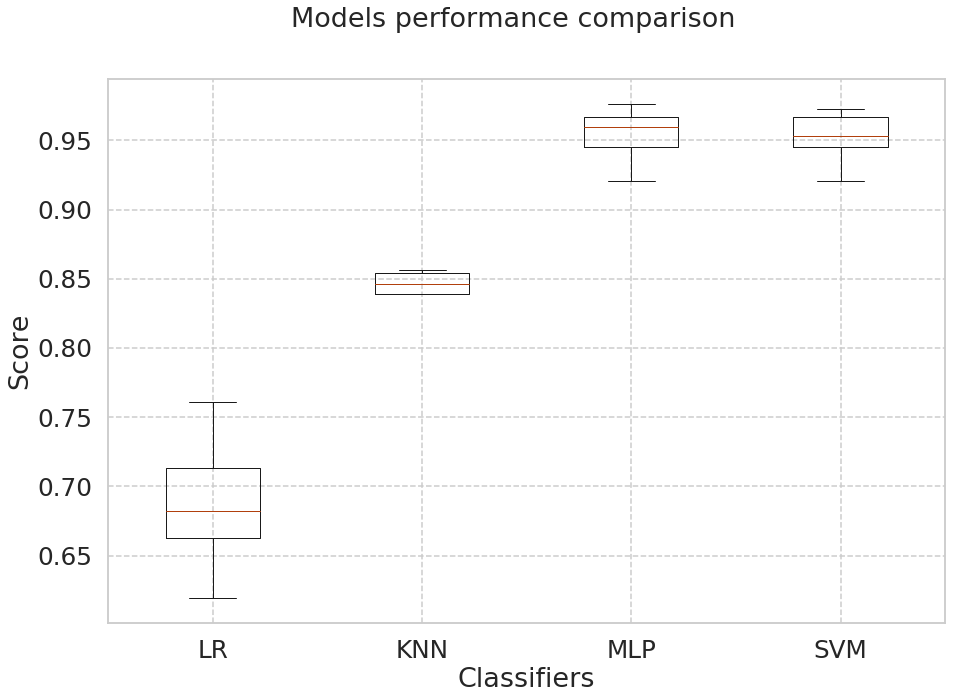
\includegraphics[width=0.7\linewidth]{Figures/K-fold_cross_validation}
	\caption{10-Fold cross validation score for LR, KNN, MLP, and SVM}
	\label{fig:k-foldcrossvalidation}
\end{figure}

MLP fitted with relu activation shows better performance compared to other classifiers. The input variable used to fit the model were all standardized to ensure the feature are equally treated in the regularization. From the  10-fold cross validation, the classifier had an average score of $95.5\%$. As shown from Figure \ref{fig:rocall}, the classier had an AUC of $1.00$ and $0.99$ for the ROC and precision-recall curves respectively. The precision-recall curve of MLP dominates with a score closed to perfect performances as compared to other classifiers.  

KNN fitted with $k$ equals to three had a general score of $85.1\%$ on the prediction of the test data. For the case of anomalies detection, KNN performed better as compared to LR. From the 10-fold cross validation score, the KNN has a score of $84.3\%$, which outperformed LR. From Figure \ref{fig:rocall}, KNN had an AUC of $0.89$ and $0.96$ in ROC and precision-recall curve respectively. 

LR fitted with parameter  C equal to $10$. The classifier had a general performance of $70.8\%$ on the test data and $69\%$ K-fold cross validation score with ten fol. From Table \ref{tab4}, the classifier identified normal class with a precision of $94.3\%$ which is slightly better as compared to KNN, and recall of LR indicates  $70.9\% $. From Figure \ref{fig:rocall},  AUC of ROC curve in LR is close to the random guess with an AUC of $69\%$ in the ROC curve. In this case, the classifier will randomly classifier a sample, hence low predictive performance. LR had the lowest predictive power in identifying the anomaly class.
%\begin{center}
%	\begin{tabular}{ |p{1.2cm}|p{1.2cm}|p{1.2cm}|p{1.2cm}|p{1.2cm}|} 
%		\hline
%		0

Across all validation tests, the LR was underperforming. In the study, accuracy techniques were used to determine the performance. Comparing the performance of the models, MLP has best accuracy score of $96.1\%$ on test data. SVM, KNN, and LR had an accuracy score of $94.9\%$, $85.1\%$ and $70.8\%$ respectively. From figure \ref{fig:rocall}, ROC and precision-recall curve of MLP is leading SVM. 

Figure \ref{fig:rocall} shows the precision-recall and ROC curves representation of the classifiers used in this study. Precision-recall curve evaluates the number of positives that the model predicted. The curve at the right corner of the precision-recall curve is considered to have more true positive predicted by the model as compared to false negative. Precision-recall curve focus on how much positive have been predicted correctly given the total positive predicted. The LR in the precision-recall curve have a drastic change, this is explained by the change of positive and negative sample in Table \ref{tab4}. The graphs below show the graphical evaluation measure of the classifiers using precision-recall and ROC curves.  

\begin{figure}[H]
	\centering
	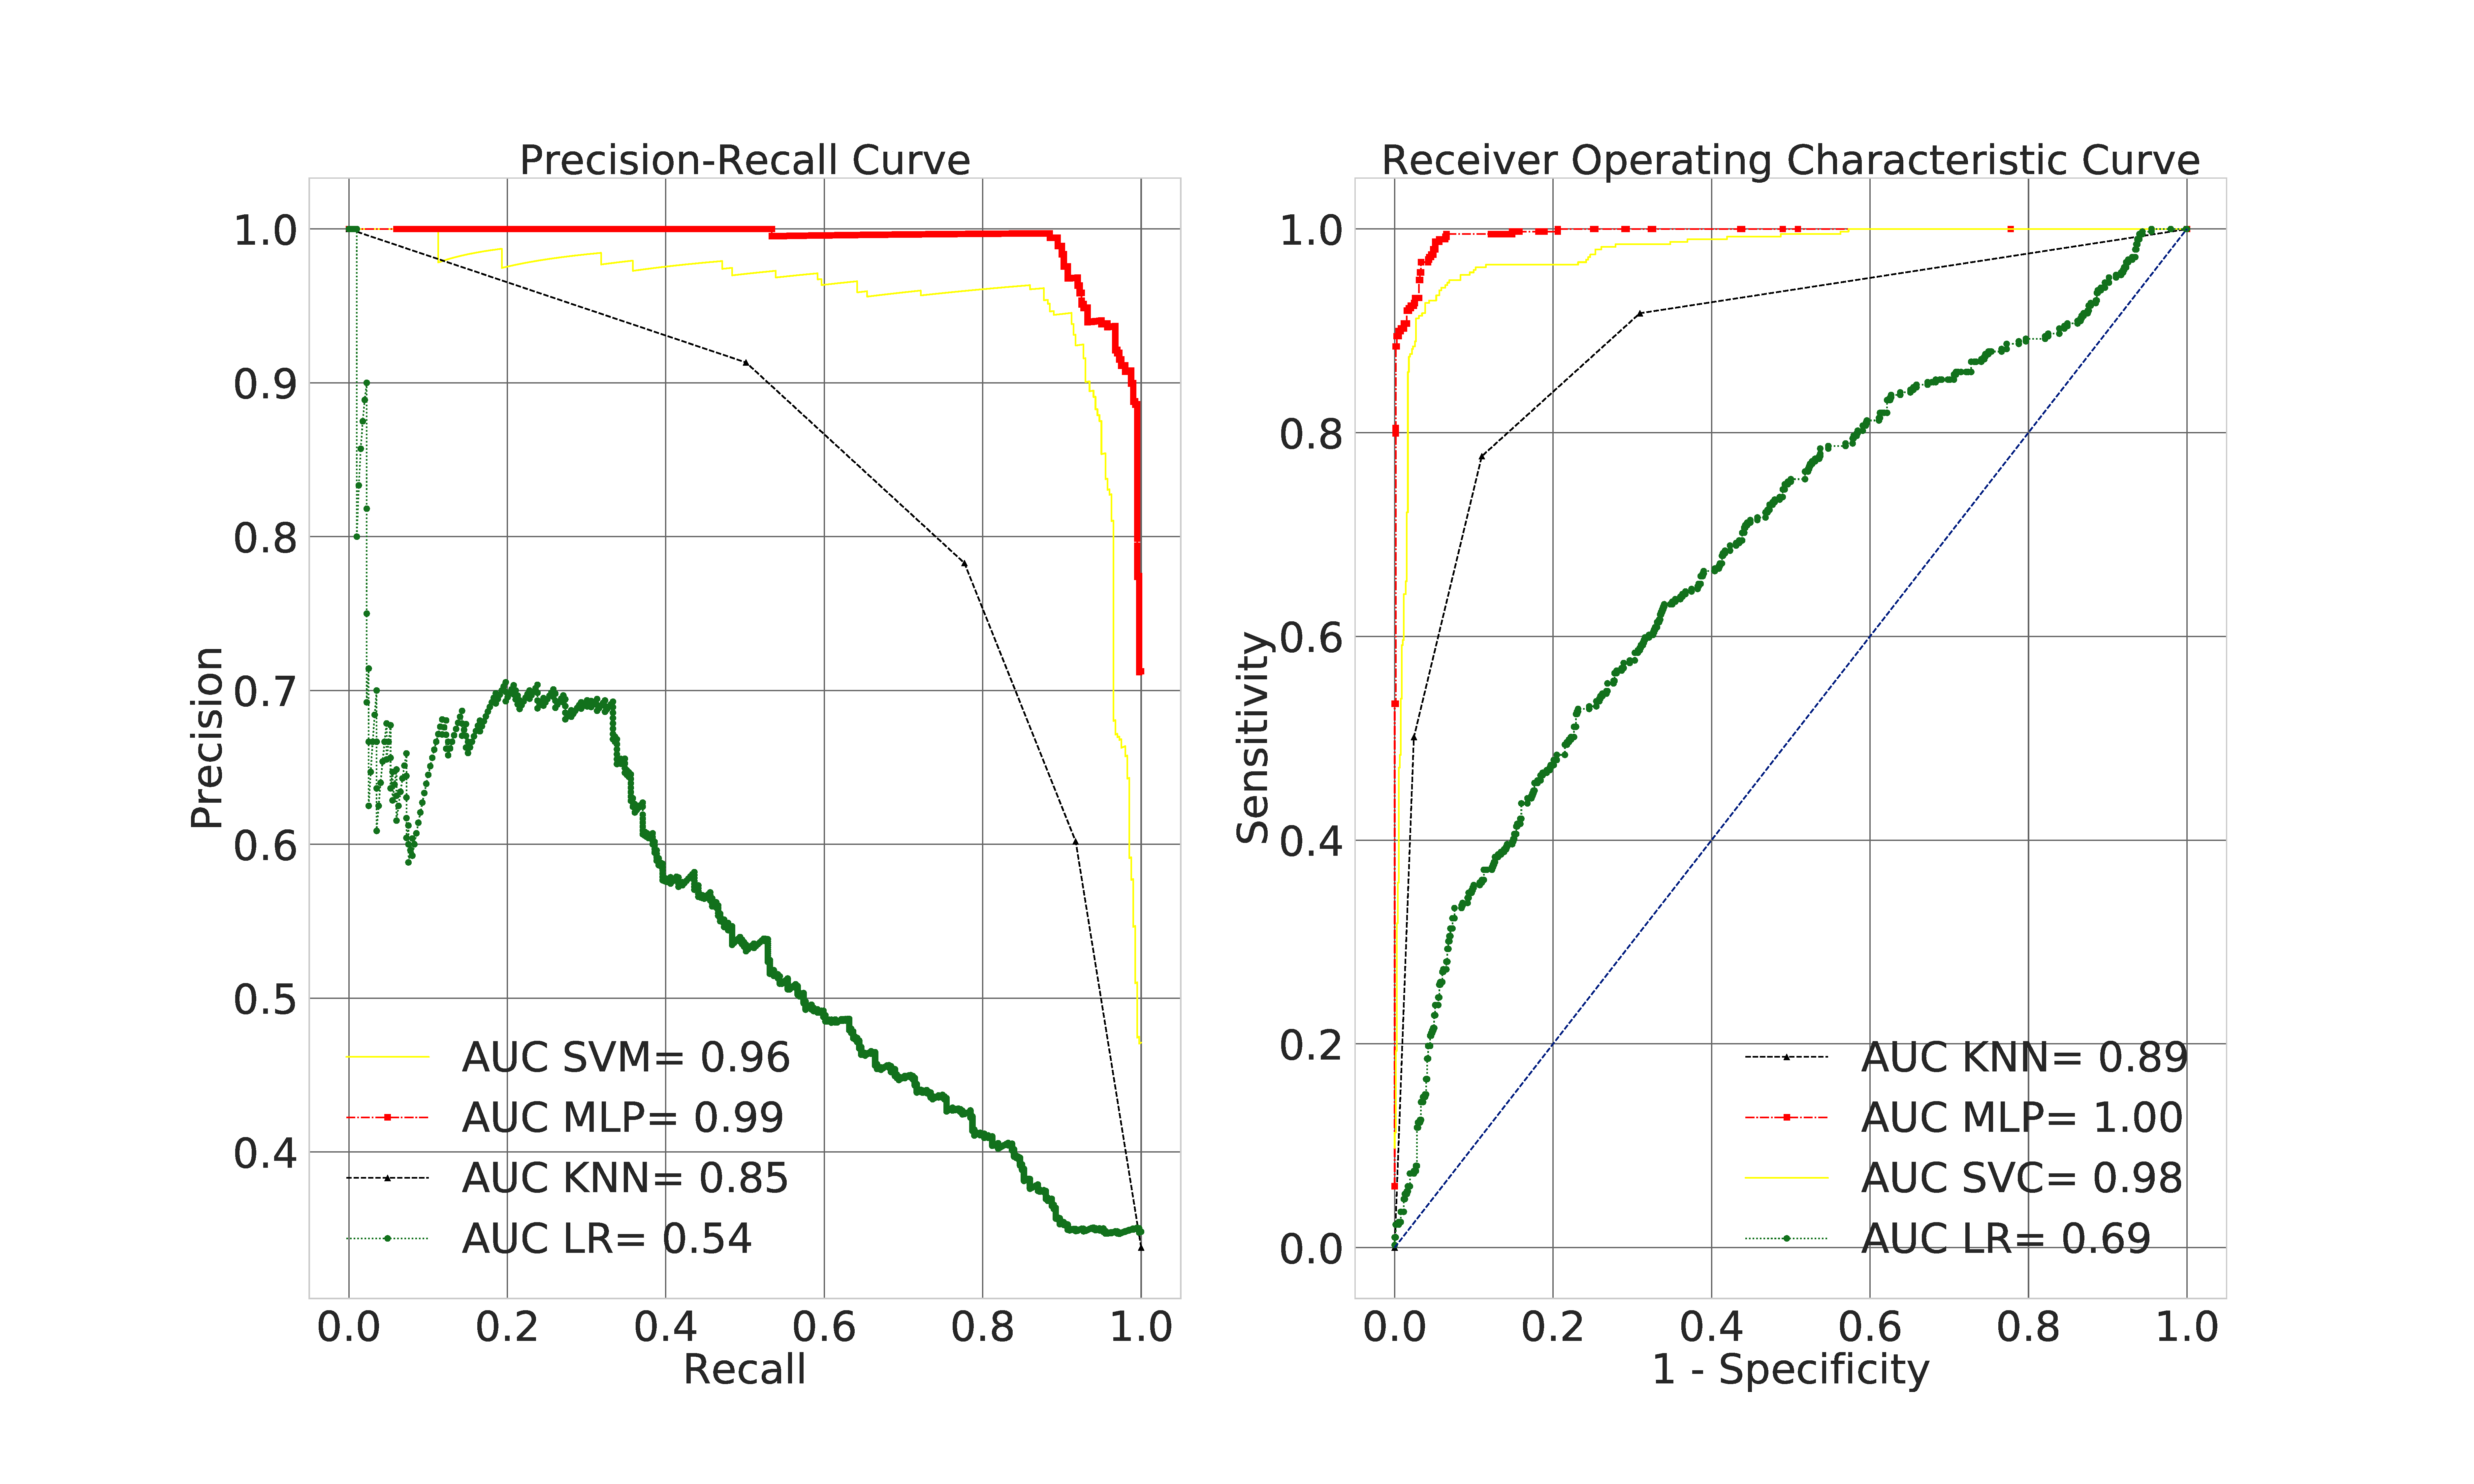
\includegraphics[width=1.2\linewidth]{Figures/ROC&PR}
	\caption{\textit{Precision-Recall curves and ROC curves of classifiers} }
\label{fig:rocall}
\end{figure}

 \subsection{Bias-Variance analysis}
Using cross validation with ten split, we observe the relationship between training score and cross validation score of different classifiers. Variation of cross validation curve is as a result of high variance and training score curve variation is as a result of high bias. Bias-variance in the model affects the performance of the model. High variance is an indication that the model learns every noise in the data. High bias indicates that the model has less information about the dataset. Regularization of bias and variance help the model to attain better predictive performance. 

From cross validation with ten fold, Figure \ref{fig:crossval} shows the cross validation and the training scores on the fitted dataset.
\begin{figure}[H]
	\centering
	\includegraphics[width=1.1\linewidth]{Figures/bias}
	\caption{Training and cross validation score curve of MLP, KNN, SVM, and LR}
		\label{fig:crossval}
\end{figure}
 In all the models the cross validation curve tends to converge with increasing training sample although SVM  and KNN the convergences is slow with increasing in the sample.  The training and cross validation curve of MLP from Figure \ref{fig:crossval} convergence faster and therefore increase in training data does not improve its performance. In LR, training score and cross validation curves converge completely with an increase in the data examples.
 
\section{CONCLUSION}

In this paper, we aimed at evaluating classification algorithm by training the model to learn and identify the anomalies in the fuel consumed dataset from a telecom base station. Four classification techniques were evaluated namely, SVM, LR, MLP, and KNN. MLP had best performance generally with an accuracy score on the test data of $96.1\%$. Although SVM outperformed other classifiers such as KNN and LR, using K- fold cross validation technique MLP performed best with score of $96.1\%$. From the confusion matrix, MLP had a best predicting power of the anomalies. LR performed better in precision score as compared to KNN, the classifier had the lowest performance as compared to all the classifiers . LR predicts more of the normal class as compared to anomaly class. The dataset was imbalance and as a result, evaluation methods which depend on both class for computation  provides wrong impression due to skew nature of the class.  ROC and Precision-recall curve used to visualize and evaluates classifiers. From Figure \ref{fig:rocall}, MLP dominates two graph with higher performance on AUC in both curves. 
For anomalies detection in the dataset, MLP had a highest performance. Anomalies is our class of interest and since the ROC curve take into consideration of the negative class, ROC curve became the most relevant graphical visualization measure for not only the study of classifier behavior but also for model selection through comparative  evaluation of different classifiers. We therefore  conclude MLP show an overall better performance compared to other classification techniques in the performance measures, that is, the classifier  best fit the training examples compared to other classifiers in terms of  anomaly detection and in evaluation performance such as K-fold cross validation, train-test split, precision-recall and ROC curves.  




\section{SUMMARY}
We fitted SVM, MLP, LR and KNN on the dataset of  fuel consumed by generator with two class, anomaly and normal class. Comparative analysis of classifiers performance using K-fold cross validation, train test spit, graphical representation techniques such as ROC and precision-recall curve were used to study the behavior of the classifier. Key indicating factors consider to evaluate the classifiers includes how well the classifier identify anomalies that exist in the test data, accuracy and AUC in ROC graph. From the results of this study, MLP performed well in all metrics evaluated. The distribution of the two class were not equal, therefore the classification accuracy was less considered in the model selection. 

\section{Acknowledgement }
The author would like to thank TeleInfra Company and Group One Holding Company for providing the dataset for this study. We wish to acknowledge Mr. OKALI DIMA Patrick from Group one holding for ensuring the data was available. Grateful for SciKit \footnote{{\tt https://scikit-learn.org/stable/modules/generated/sklearn.svm.SVC.html}} learn library as this work has been made possible from the use of their library packages.
\section{References} \label{sec:references}
 \bibliographystyle{elsarticle-harv} 
 \bibliography{ref.bib} %{<your bibdatabase>}
%% else use the following coding to input the bibitems directly in the
%% TeX file.
% \begin{thebibliography}{00}
% 
% %% \bibitem[Author(year)]{label}
% %% Text of bibliographic item
% 
% \bibitem[ ()]{}
% 
% \end{thebibliography}
\end{document}
\endinput
%%
%% End of file `elsarticle-template-harv.tex'.
